% Standalone: compile twice with pdfLaTeX. The diagrams are drawn in TikZ.
\documentclass[11pt,a4paper]{article}
\usepackage[T1]{fontenc}
\usepackage{lmodern}
\usepackage[english]{babel}
\usepackage{microtype}
\usepackage{amsmath,amssymb,amsthm,mathtools}
\usepackage{geometry}
\usepackage{tikz}
\usetikzlibrary{arrows.meta}
\usepackage[hidelinks]{hyperref}
\geometry{a4paper,margin=24mm,headheight=14pt}
\setlength{\parindent}{0pt}
\setlength{\parskip}{4pt plus 1pt minus 1pt}
\allowdisplaybreaks[1]
\raggedbottom
\newcommand{\R}{\mathbb{R}}
\newcommand{\T}{\mathbb{T}}
\newcommand{\Z}{\mathbb{Z}}
\newcommand{\D}{\mathcal{D}}
\newcommand{\A}{\mathcal{A}}
\newcommand{\U}{\mathcal{U}}
\newcommand{\PP}{\mathbb{P}}
\newcommand{\EE}{\mathbb{E}}
\newcommand{\norm}[1]{\lVert #1\rVert}
\DeclareMathOperator{\Law}{Law}
\newtheorem*{cancellation}{Theorem 3.1 (Cancellation estimate)}
\newtheorem*{doubling}{Lemma 6.3 (Doubling bound)}
\newtheorem*{critical}{Lemma 6.4 (Critical scales)}
\newcommand{\seminarurl}{https://kaminoite.github.io/jordilluisfigueras/ReadingGroupUBUPCPositiveMetricEntropy}
\newcommand{\paperurl}{https://github.com/openai/math/blob/main/preprints/Positive-Metric-Entropy-for-the-Standard-Map-at-Large-Parameters-September-23-2026/paper.pdf}
\hypersetup{pdftitle={Positive Metric Entropy for the Standard Map. Day 2: Dyadic scales and laws of growth semimetrics},pdfauthor={Reading Group UB-UPC}}

% The figures use the same colours in the torus and in the space of arrays.
\definecolor{water}{HTML}{85B7C7}
\definecolor{waterline}{HTML}{437888}
\definecolor{goldarea}{HTML}{F7D875}
\definecolor{goldline}{HTML}{876019}
\definecolor{affine}{HTML}{693C79}
\definecolor{outline}{HTML}{293D46}

% Orthographic projection of a torus. The two outlines are the parallel
% curves of its projected centre circle. Angles are in degrees.
\tikzset{declare function={
  torx(\u,\v)=(1.65+0.43*cos(\v))*cos(\u);
  tory(\u,\v)=0.53*(1.65+0.43*cos(\v))*sin(\u)+0.848*0.43*sin(\v);
  ellnorm(\u)=sqrt((0.53*cos(\u))^2+(sin(\u))^2);
  rimx(\u,\r)=1.65*cos(\u)+\r*0.53*cos(\u)/ellnorm(\u);
  rimy(\u,\r)=0.53*1.65*sin(\u)+\r*sin(\u)/ellnorm(\u);
  vlow(\u,\v)=max(\v,atan2(0.53,-0.848*sin(\u))-90);
  vhigh(\u,\v)=min(\v,atan2(0.53,-0.848*sin(\u))+90);
  shiftq(\t)=\t+2/pi*sin(360*\t);
}}
\newcommand{\torusrim}[1]{plot[smooth,variable=\t,domain=0:360,samples=65]
  ({rimx(\t,#1)},{rimy(\t,#1)}) -- cycle}
\newcommand{\toruspatch}{plot[smooth,variable=\t,domain=0:360,samples=55]
  ({torx(302+32*cos(\t),25+48*sin(\t))},
   {tory(302+32*cos(\t),25+48*sin(\t))}) -- cycle}
\newcommand{\torusgrid}{%
  \foreach \az in {0,20,...,340}{
    \pgfmathsetmacro{\centre}{atan2(0.53,-0.848*sin(\az))}
    \pgfmathsetmacro{\firstangle}{\centre-89.9}
    \pgfmathsetmacro{\lastangle}{\centre+89.9}
    \draw plot[smooth,variable=\t,domain=\firstangle:\lastangle,samples=22]
      ({torx(\az,\t)},{tory(\az,\t)});
  }
  \foreach \el/\firstangle/\lastangle in
    {-22/195/345,0/180/360,32/157/383,68/0/360,110/0/360,147/-24/204,180/0/180,201/14/166}{
    \draw plot[smooth,variable=\t,domain=\firstangle:\lastangle,samples=48]
      ({torx(\t,\el)},{tory(\t,\el)});
  }}
% Visible part of the parameter rectangle 210 <= u <= 390, #1 <= v <= #2.
\newcommand{\eventpatch}[2]{%
  plot[variable=\t,domain=210:390,samples=60]
    ({torx(\t,vlow(\t,#1))},{tory(\t,vlow(\t,#1))})
  -- plot[variable=\t,domain=0:1,samples=25]
    ({torx(390,vlow(390,#1)+\t*(vhigh(390,#2)-vlow(390,#1)))},
     {tory(390,vlow(390,#1)+\t*(vhigh(390,#2)-vlow(390,#1)))})
  -- plot[variable=\t,domain=390:210,samples=60]
    ({torx(\t,vhigh(\t,#2))},{tory(\t,vhigh(\t,#2))})
  -- plot[variable=\t,domain=0:1,samples=25]
    ({torx(210,vhigh(210,#2)-\t*(vhigh(210,#2)-vlow(210,#1)))},
     {tory(210,vhigh(210,#2)-\t*(vhigh(210,#2)-vlow(210,#1)))})
  -- cycle}
\newcommand{\drawtorus}[1][\toruspatch]{%
  \path[shade,top color=water!66,bottom color=water!88!waterline,even odd rule]
    \torusrim{0.43} \torusrim{-0.43};
  \begin{scope}[even odd rule]
    \clip \torusrim{0.43} \torusrim{-0.43};
    \begin{scope}[draw=waterline!65,line width=0.27pt]\torusgrid\end{scope}
    \filldraw[fill=goldarea,draw=goldline,line width=0.65pt] #1;
    \begin{scope}
      \clip #1;
      \begin{scope}[draw=goldline!55,line width=0.28pt]\torusgrid\end{scope}
    \end{scope}
  \end{scope}
  \draw[waterline,line width=0.65pt] \torusrim{0.43} \torusrim{-0.43};}

% In the two-coordinate example a fixed interval of q_1 produces a curved
% strip in (x,y). Periodic copies are clipped to the unit square.
\newcommand{\phasewindow}[3]{%
  \path[fill=water!22] (0,0) rectangle (1,1);
  \begin{scope}
    \clip (0,0) rectangle (1,1);
    \foreach \k in {-2,-1,0,1,2}{
      \path[fill=goldarea,draw=goldline,line width=.48pt]
        plot[variable=\x,domain=.25:.75,samples=64] (\x,{#1-shiftq(\x)+\k})
        -- plot[variable=\x,domain=.75:.25,samples=64] (\x,{#2-shiftq(\x)+\k})
        -- cycle;
    }
    \ifnum#3=1
      \foreach \k in {-1,0,1}{
        \draw[affine,line width=1.3pt] plot[variable=\x,domain=.25:.75,samples=70]
          (\x,{-2/pi*sin(360*\x)+\k});
      }
    \fi
  \end{scope}
  \draw[outline,line width=.65pt] (0,0) rectangle (1,1);
  \node[below left,inner sep=1.2pt,font=\scriptsize] at (0,0) {$0$};
  \node[below,inner sep=1.2pt,font=\scriptsize] at (1,0) {$1$};
  \node[left,inner sep=1.2pt,font=\scriptsize] at (0,1) {$1$};
  \node[below,inner sep=1.2pt,font=\footnotesize] at (.5,0) {$x$};
  \node[left,inner sep=2pt,font=\footnotesize] at (0,.5) {$y$};}
\newcommand{\testwindow}[1]{%
  \pgfmathsetmacro{\cutc}{ln(1+sqrt(2))/ln(8)}
  \pgfmathsetmacro{\cutb}{ln(2+sqrt(5))/ln(8)}
  \pgfmathsetmacro{\cute}{ln(3+sqrt(10))/ln(8)}
  \path[fill=water!22,draw=waterline!80,line width=.5pt] (0,0) rectangle (\cute,\cute);
  \ifnum#1=1
    \path[fill=goldarea,draw=goldline,line width=.65pt] (0,0) rectangle (\cutc,\cutc);
  \else
    \path[fill=goldarea,draw=goldline,line width=.65pt] (0,\cutb) rectangle (\cutc,\cute);
  \fi
  \draw[affine,dashed,line width=.65pt] (0,0)--(1,1);
  \ifnum#1=1 \draw[affine,line width=1.4pt] (0,0)--(\cutc,\cutc);\fi
  \draw[outline,line width=.65pt] (0,0) rectangle (1,1);
  \node[below left,inner sep=1.2pt,font=\scriptsize] at (0,0) {$0$};
  \node[below,inner sep=1.2pt,font=\scriptsize] at (1,0) {$1$};
  \node[left,inner sep=1.2pt,font=\scriptsize] at (0,1) {$1$};
  \node[below,inner sep=1.2pt,font=\scriptsize] at (\cutc,0) {$c$};
  \ifnum#1=1
    \node[left,inner sep=1.5pt,font=\scriptsize] at (0,\cutc) {$c$};
  \else
    \node[left,inner sep=1.5pt,font=\scriptsize] at (0,\cutb) {$b$};
    \node[left,inner sep=1.5pt,font=\scriptsize] at (0,\cute) {$e$};
  \fi}

\title{\vspace{-1.4em}\textbf{Positive Metric Entropy for the Standard Map}\\[4pt]
  \large Day 2. Dyadic scales and laws of growth semimetrics}
\author{Reading Group UB-UPC}
\date{25 November 2026}

\begin{document}
\maketitle
\vspace{-1.2em}
\begin{abstract}
\noindent
How can a mean growth shortfall that tends to zero at every fixed time begin
to increase at long times? We derive the doubling bound for $e_n(K)$ and select
the critical dyadic scales. We interpret the law of a growth array as torus area,
compute two examples, and construct the three measures of Section~6 of the preprint.
\end{abstract}

\section{From the derivative to a distance on time}
Write $m$ for normalized area on $\T^2=(\R/\Z)^2$. With $K=2\pi k>0$, set
\[
 V(x)=\frac{K}{2\pi}\sin(2\pi x),\qquad
 f_k(x,y)=\bigl(x+y+V(x),\,y+V(x)\bigr)\pmod{\Z^2},\qquad M=K+4.
\]
For $z_i=f_k^i(z)=(x_i,y_i)$ put $q_i=x_i$. Since $q_{i-1}=x_i-y_i$,
the torus coordinates $(q_i,q_{i-1})$ give $q_{i+1}=2q_i+V(q_i)-q_{i-1}$ modulo one.
The derivative in these coordinates and its transfer products are
\[
 A_i=\begin{pmatrix}2+K\cos(2\pi q_i)&-1\\1&0\end{pmatrix},
 \qquad T_{a,b}(z)=A_{b-1}\cdots A_a\quad (a<b).
\]
Set $T_{a,a}=I$ and $T_{b,a}=T_{a,b}^{-1}$. The singular values of a determinant-one
$2\times2$ matrix are $D,D^{-1}$ with $D\ge1$. In the Euclidean operator norm,
$\norm{A_i^{\pm1}}\le M$, so $1\le\norm{T_{a,b}}=\norm{T_{b,a}}\le M^{|b-a|}$.
The growth array satisfies
\begin{equation}\label{eq:g}
 g(a,b;z)=\log_M\norm{T_{a,b}(z)},\qquad 0\le g(a,b;z)\le |b-a|.
\end{equation}
For fixed $z$, this is a semimetric on $\Z$. Its diagonal is zero, equality of the
forward and backward norms gives symmetry, and $T_{a,c}=T_{b,c}T_{a,b}$ gives the
triangle inequality. Distinct times can have zero distance.

\subsection*{Two orders of limits}
The mean shortfall is $e_n(K)=\int_{\T^2}(1-g(0,n;z)/n)\,dm(z)$. A shortfall near
zero means nearly maximal growth in units of $\log M$. For any fixed $0<\eta<1$,
the set $|2+K\cos(2\pi q)|<M^{1-\eta}$ has length tending to zero. A union bound
over $n$ visits, followed by the cone estimate from Day~1, gives $e_n(K)\to0$
for each fixed $n$ as $K\to\infty$.

The goal is $m\{z:\lambda_+(z)>0\}>0$ for all large $K$. Suppose, towards a
contradiction, that $K_j\to\infty$ have zero metric entropy. By Pesin's formula
the top Lyapunov exponent vanishes almost everywhere at each $K_j$. Since
$g(0,n;z)/n\to\lambda_+(z)/\log M$ and this ratio lies in $[0,1]$, bounded
convergence gives the second limit below.
\[
 \boxed{\quad \lim_{j\to\infty}e_n(K_j)=0\quad(n\text{ fixed}),\qquad
             \lim_{n\to\infty}e_n(K_j)=1\quad(j\text{ fixed}).\quad}
\]
The two limits are compatible. How quickly can the shortfall increase with $n$?

\newpage
\section{How much shortfall can one doubling create?}
We use $\EE$ and $\PP$ for expectation and probability with respect to $m$.
Shifting every integer time by $i$ has the same effect on $g$ as replacing $z$
by $f_k^i(z)$. Area invariance therefore makes the array stationary.

\begin{cancellation}
There are $\delta,\gamma>0$, $C_{\rm can}<\infty$ and $M_0$ such that for
$M\ge M_0$, $i\in\Z$ and $n\ge1$,
\[
 \PP\!\left\{\begin{aligned}
 &\min\{g(i-n,i),\,g(i,i+n)\}\ge(1-\delta)n,\\
 &g(i-n,i+n)\le\delta n
 \end{aligned}\right\}\le C_{\rm can}e^{-\gamma n}.
\]
\end{cancellation}
Each half can have nearly maximal growth while the product across both halves
has very little growth. The estimate bounds the area of initial states giving
this near-complete cancellation at a specified centre and length.

\begin{doubling}
For every sufficiently large $K$ and every integer $n\ge1$, an absolute
constant $C$ gives
\begin{equation}\label{eq:doubling}
 \boxed{\qquad e_n\le e_{2n}\le C\bigl(e_n+n^{-1}\bigr).\qquad}
\end{equation}
\end{doubling}
\begin{proof}
Fix a centre $i$ and write $L=i-n$, $R=i+n$. Introduce the two losses
\[
 D=n-\min\{g(L,i),g(i,R)\},\qquad
 \ell=g(L,i)+g(i,R)-g(L,R).
\]
Here $D$ is the larger of the two half-interval shortfalls in units of time.
The triangle defect $\ell\ge0$ is the additional loss upon joining the halves.
Stationarity gives the exact identity and the estimate
\begin{equation}\label{eq:defect}
 e_{2n}-e_n=\frac{\EE\ell}{2n},\qquad \EE D\le 2ne_n .
\end{equation}
This proves the lower bound. For the upper bound, Lemma~6.2 of the preprint
truncates a cancellation to radius $1\le s\le n$. For a uniform constant $A$ it gives
\[
 g(i,i\pm s)\ge s-D,\qquad
 g(i-s,i+s)\le 2s-\min\{\ell,\,2s-2D\}+A.
\]
If $\ell>H(1+D)$, take $s=\lfloor\ell/2\rfloor$. Choosing the absolute constant
$H$ large ensures $1\le s\le n$ and $2D+A\le\delta s$. Since $2s\le\ell$,
\[
 \min\{g(i-s,i),g(i,i+s)\}\ge(1-\delta)s,\qquad g(i-s,i+s)\le\delta s.
\]
For each possible $s$, Theorem~3.1 bounds the probability of this event.
Since $\ell<2s+2$ on that part, summing over $s$ yields
\[
 \EE\ell \le H(1+\EE D)+C_{\rm can}\sum_{s\ge1}(2s+2)e^{-\gamma s}.
\]
Substitution in \eqref{eq:defect} proves \eqref{eq:doubling}.
\end{proof}

The other dynamical input from Day~1, Theorem~5.1, compares observations near
opposite ends of a rapidly expanding interval. Its role comes later, when such
an interval constrains the possible shapes of a limiting array.

\newpage
\section{Choosing the initial and terminal scales}
Suppress $K$ in $e_n$ and let it run along the hypothetical sequence $K_j$.
All the scales selected below are powers of two.
\begin{critical}
There are $n_0=n_0(K)<N=N(K)$ and $\varepsilon=e_N(K)$ such that
\begin{equation}\label{eq:critical}
 n_0\longrightarrow\infty,\qquad \varepsilon\longrightarrow0,\qquad
 \varepsilon n_0\longrightarrow\infty .
\end{equation}
For each fixed integer $r$, once the lengths are integers,
\begin{equation}\label{eq:shifts}
 e_{2^r n_0}=o(\varepsilon),\qquad e_{2^r N}=O_r(\varepsilon).
\end{equation}
\end{critical}
\begin{proof}
Fixed-time growth permits a diagonal choice of $n_0\to\infty$ so slowly that
$e_{n_0}\to0$. Put $\theta=(e_{n_0}+n_0^{-1})^{1/2}$. At a fixed parameter
$e_n\to1$, so there is a first dyadic $N\ge n_0$ with $e_N>\theta$.
Eventually $e_{n_0}<\theta<1$, hence $N>n_0$. Its predecessor satisfies
$e_{N/2}\le\theta$. The doubling bound gives
\[
 \theta<\varepsilon=e_N\le C(\theta+n_0^{-1})\to0,\qquad
 n_0\varepsilon\ge n_0\theta\ge\sqrt{n_0}.
\]
For fixed $r\ge0$ iterate \eqref{eq:doubling}. At $n_0$ the resulting bound is
$C_r(e_{n_0}+n_0^{-1})=C_r\theta^2=o(\varepsilon)$, and at $N$ it is
$C_r(\varepsilon+N^{-1})=O_r(\varepsilon)$. For $r<0$ dyadic monotonicity
bounds the shifted shortfalls by $e_{n_0}$ and $e_N$, respectively.
\end{proof}
Thus the terminal shortfall equals one in units of $\varepsilon$, while every
fixed dyadic multiple of the initial scale still has negligible shortfall in
those units. In particular $N/n_0\to\infty$.

\section{A compact space for comparing scales}
Let $\D=\Z[1/2]=\{j/2^r:j\in\Z,\ r\ge0\}$. Section~6.3 of the preprint takes $X$
to consist of all semimetrics $d$ on $\D$ such that $d(s,t)\le |s-t|+2$.
Use the topology of pointwise convergence on $\D^2$. Then
\[
 X\ \subseteq\ \prod_{(s,t)\in\D^2}[0,|s-t|+2]
\]
is closed because each diagonal, symmetry and triangle condition is closed.
The product is compact and metrizable since there are countably many pairs.
In particular a sequence in $X$ has a subsequence converging on every dyadic pair.

The affine family and its complement are
\begin{equation}\label{eq:affine}
 \A=\{d_w:0\le w\le1\},\qquad d_w(s,t)=w|t-s|,\qquad \U=X\setminus\A .
\end{equation}
The bound in $X$ at arbitrarily large separations forces $w\le1$. The map
$w\mapsto d_w$ identifies $\A$ with a closed interval, with inverse $d\mapsto d(0,1)$
on $\A$. At $w=0$ all times have zero mutual distance.

A concrete point of $\U$ is the folded array $d(s,t)=\bigl||s|-|t|\bigr|$.
It is the pullback of the usual distance under $t\mapsto|t|$. The distances
from $0$ to $-1$ and from $0$ to $1$ both equal one, while $d(-1,1)=0$.
An affine array with those first two distances would have $w=1$ and $d(-1,1)=2$.

\newpage
\section{One point of the torus gives one array}
Fix $K$ and a positive integer $n$. The map into $X$ is
\begin{equation}\label{eq:array}
 G_n:\T^2\longrightarrow X,\qquad G_n(z)=g_n(\cdot,\cdot;z),\qquad
 g_n(s,t;z)=\frac{g(\lfloor ns\rfloor,\lfloor nt\rfloor;z)}{n}.
\end{equation}
The floor function pulls the integer-time semimetric back to $\D$. By \eqref{eq:g},
$g_n(s,t;z)\le |s-t|+1/n$, so $G_n(z)\in X$. Every coordinate varies continuously
with $z$, hence $G_n$ is continuous for the product topology.

For instance, when $n$ is even, the three coordinates at
$(0,\tfrac12),(\tfrac12,1),(0,1)$ record the growth on the two halves and on the
whole orbit segment. All three use the same initial point and the same denominator $n$.

\subsection*{What does the law measure?}
Choose $z$ according to $m$. The resulting $X$-valued random variable has distribution
\begin{equation}\label{eq:law}
 \boxed{\quad\Law(g_n)=(G_n)_*m,\qquad
 \Law(g_n)(B)=m\bigl(G_n^{-1}(B)\bigr)\quad(B\subset X\text{ Borel}).\quad}
\end{equation}
\begin{figure}[ht]
\centering
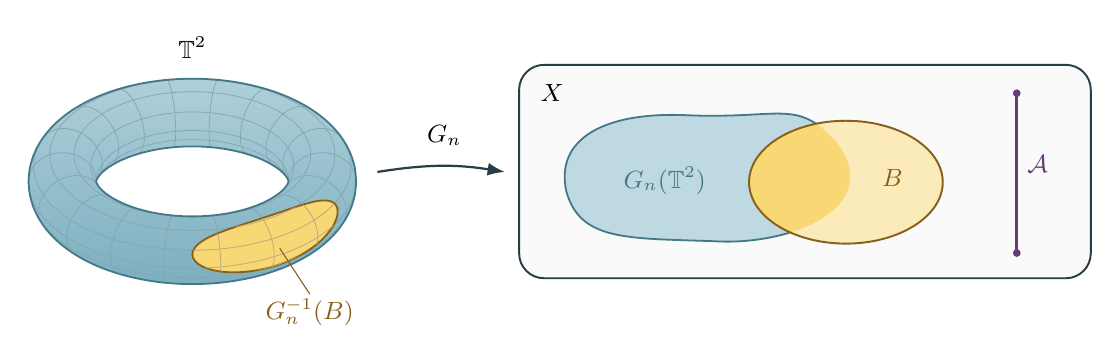
\begin{tikzpicture}[x=1cm,y=1cm,>={Latex[length=2.2mm]},font=\small]
  \begin{scope}[shift={(2.15,0)}]\drawtorus\end{scope}
  \node at (2.15,1.7) {$\T^2$};
  \draw[goldline,thin] (3.26,-.85)--(3.64,-1.43);
  \node[below,text=goldline,inner sep=1.4pt] at (3.64,-1.43) {$G_n^{-1}(B)$};
  \draw[->,outline,line width=.8pt] (4.50,.12) to[bend left=9] (6.12,.12);
  \node at (5.35,.58) {$G_n$};
  \begin{scope}[shift={(6.3,-1.23)}]
    \path[draw=outline,fill=black!2,line width=.7pt,rounded corners=9pt]
      (0,0) rectangle (7.26,2.71);
    \node at (.42,2.35) {$X$};
    \path[draw=waterline,fill=water!53,line width=.65pt]
      (.6,1.1) .. controls (.45,1.77) and (1.08,2.12) .. (2.14,2.07)
      .. controls (3.35,2.02) and (3.52,2.29) .. (4.04,1.72)
      .. controls (4.65,.89) and (3.44,.41) .. (2.48,.47)
      .. controls (1.37,.51) and (.78,.47) .. cycle;
    \def\testoval{(4.15,1.22) ellipse [x radius=1.23,y radius=.78]}
    \path[fill=goldarea!50] \testoval;
    \begin{scope}
      \clip (.6,1.1) .. controls (.45,1.77) and (1.08,2.12) .. (2.14,2.07)
        .. controls (3.35,2.02) and (3.52,2.29) .. (4.04,1.72)
        .. controls (4.65,.89) and (3.44,.41) .. (2.48,.47)
        .. controls (1.37,.51) and (.78,.47) .. cycle;
      \fill[goldarea] \testoval;
    \end{scope}
    \draw[goldline,line width=.7pt] \testoval;
    \node[text=waterline] at (1.85,1.24) {$G_n(\T^2)$};
    \node[text=goldline] at (4.74,1.27) {$B$};
    \draw[affine,line width=1.1pt] (6.32,.32)--(6.32,2.35);
    \fill[affine] (6.32,.32) circle (1.4pt) (6.32,2.35) circle (1.4pt);
    \node[right,text=affine] at (6.33,1.45) {$\A$};
  \end{scope}
\end{tikzpicture}
\caption{Read the drawing from right to left to evaluate the law. Choose $B$ in
$X$ and measure the gold region on the torus. Only $B\cap G_n(\T^2)$ contributes.
The shapes in $X$ are schematic.}
\label{fig:law}
\end{figure}

Equivalently, each bounded Borel observable $F:X\to\R$ satisfies
\[
 \int_X F(d)\,d\Law(g_n)(d)=\int_{\T^2}F(G_n(z))\,dm(z).
\]
Taking $F(d)=1-d(0,1)$ recovers exactly $e_n(K)$. Taking the indicator of
$B_\eta=\{d:d(0,1)\le1-\eta\}$ measures the area of initial states losing at least
the fraction $\eta$ of maximal growth. For $0<\eta<1$ this area is at most
$e_n(K)/\eta$, by Markov's inequality on the sampled arrays.

The law also records joint events. For example, the three entries in the
folded configuration on the preceding page give the Borel test
\[
 B_{\rm fold}=\{d:\min(d(-1,0),d(0,1))\ge1-\delta,\ d(-1,1)\le\delta\}.
\]
Theorem~3.1 with centre $i=0$ reads $\Law(g_n)(B_{\rm fold})\le
C_{\rm can}e^{-\gamma n}$. The same $z$ must satisfy all three inequalities.

\newpage
\subsection*{Seeing an affine segment in two coordinates}
The law is defined at every parameter. Take $n=1$ and $K=4$, so $M=8$ and the
shaded areas are easy to compute. Record two entries by $\pi(d)=(d(0,1),d(1,2))$. Then
\[
 (\pi\circ G_1)(x,y)=(u(q_0),u(q_1)),\qquad
 u(q)=p(|2+4\cos(2\pi q)|),\qquad p(a)=\log_8\frac{a+\sqrt{a^2+4}}2 .
\]
Indeed the larger singular value $D$ of a one-step matrix satisfies
$D-D^{-1}=|2+4\cos(2\pi q)|$. For fixed $q_0=x$, the map from $y$ to
$q_1=x+y+(2/\pi)\sin(2\pi x)\pmod1$ is a circle translation. Thus $q_0,q_1$
are independent and uniform under $m$, and a rectangle of observed values
has probability equal to the product of two one-dimensional lengths.

Put $c=p(2)$, $b=p(4)$ and $e=p(6)$. The conditions $u(q)\le c$ and
$b\le u(q)\le e$ give, respectively, $q\in I=[1/4,3/4]$ and
$q\in J=[-1/6,1/6]\pmod1$. For $B_i=\pi^{-1}(R_i)$ this gives
\[
\begin{array}{c@{\qquad}c@{\qquad}c}
 R_1=[0,c]^2 & (q_0,q_1)\in I\times I & \Law(g_1)(B_1)=\tfrac12\cdot\tfrac12=\tfrac14,\\[3pt]
 R_2=[0,c]\times[b,e] & (q_0,q_1)\in I\times J & \Law(g_1)(B_2)=\tfrac12\cdot\tfrac13=\tfrac16 .
\end{array}
\]
\begin{figure}[ht]
\centering
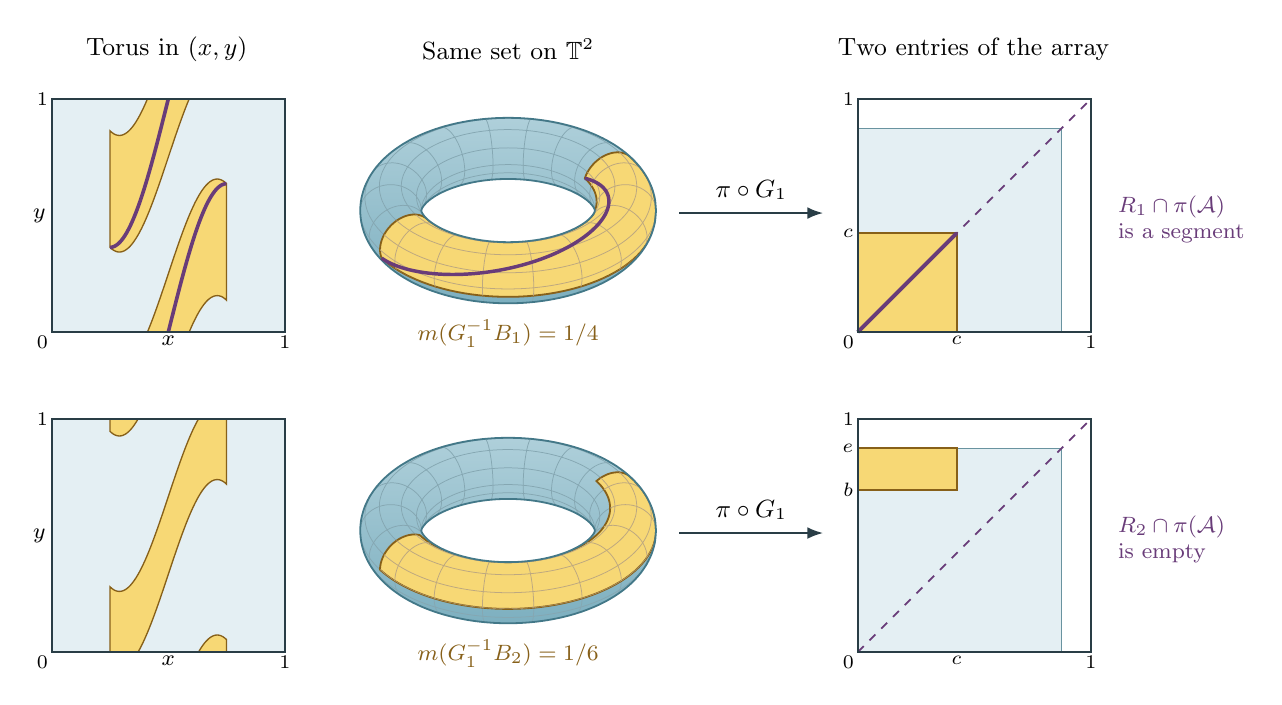
\begin{tikzpicture}[x=1cm,y=1cm,scale=1.05,>={Latex[length=2mm]},font=\small]
  \node at (1.42,3.42) {Torus in $(x,y)$};
  \node at (5.55,3.42) {Same set on $\T^2$};
  \node at (11.18,3.42) {Two entries of the array};
  \foreach \row/\baseline in {1/0,2/-3.87}{
    \begin{scope}[shift={(.03,\baseline)},x=2.82cm,y=2.82cm]
      \ifnum\row=1 \phasewindow{.25}{.75}{1}\else \phasewindow{-1/6}{1/6}{0}\fi
    \end{scope}
    \begin{scope}[shift={(5.55,{\baseline+1.47})},x=.86cm,y=.86cm]
      \ifnum\row=1
        % u=360 q_0+120, v=360 q_1-110. The marked branch has q_1=q_0.
        \drawtorus[\eventpatch{-20}{160}]
        \draw[affine,line width=1.25pt] plot[smooth,variable=\t,domain=210:390,samples=55]
          ({torx(\t,\t-230)},{tory(\t,\t-230)});
      \else
        % Rotate the second angular coordinate to expose the second patch.
        % u=360 q_0+120, v=360 q_1+60.
        \drawtorus[\eventpatch{0}{120}]
      \fi
    \end{scope}
    \begin{scope}[shift={(9.78,\baseline)},x=2.82cm,y=2.82cm]
      \testwindow{\row}
    \end{scope}
    \draw[->,outline,line width=.7pt] (7.62,{\baseline+1.44})--(9.36,{\baseline+1.44});
    \node[above] at (8.49,{\baseline+1.48}) {$\pi\circ G_1$};
    \ifnum\row=1
      \node[text=goldline,font=\footnotesize] at (5.55,{\baseline-.02}) {$m(G_1^{-1}B_1)=1/4$};
      \node[align=left,anchor=west,text=affine,font=\footnotesize] at (12.81,{\baseline+1.36})
        {$R_1\cap\pi(\A)$\\is a segment};
    \else
      \node[text=goldline,font=\footnotesize] at (5.55,{\baseline-.02}) {$m(G_1^{-1}B_2)=1/6$};
      \node[align=left,anchor=west,text=affine,font=\footnotesize] at (12.81,{\baseline+1.36})
        {$R_2\cap\pi(\A)$\\is empty};
    \fi
  }
\end{tikzpicture}
\caption{The two views on the left show the same gold set. The drawn tori use
angular coordinates $(q_0,q_1)$ with the origin rotated to show each set.
Areas use $dm=dx\,dy=dq_0\,dq_1$. The blue square on the right is the image $[0,e]^2$. The diagonal is
$\pi(\A)=\{(w,w):0\le w\le1\}$. In the top row one branch over its highlighted
segment is $q_1=q_0$, or $y=-(2/\pi)\sin(2\pi x)\pmod1$ for $x\in I$.
Opposite edges of each torus square are identified.}
\label{fig:exact}
\end{figure}

In $X$ the exact intersection is $B_1\cap\A=\{d_w:0\le w\le c\}$. The purple
curve on the torus tests equality of the two displayed entries. Global affinity
would require $g_1(s,t;z)=w|t-s|$ at \emph{every} dyadic pair. Indeed, at any
finite $n$, two distinct dyadic times in the same floor cell have $g_n(s,t;z)=0$,
so a full finite-scale array cannot equal $d_w$ with $w>0$.

\newpage
\section{Putting the laws at different scales together}
Return to the sequence in Lemma~6.4. Let $p=\log_2(N/n_0)$ and
$n_j=2^j n_0$, $0\le j\le p$, so $n_p=N$. Each $\Law(g_{n_j})$ is a
probability measure on the same compact space $X$. The three measures of
equation~(6.14) in the preprint are
\begin{equation}\label{eq:measures}
 \boxed{\quad
 \xi_K=\varepsilon^{-1}\Law(g_{n_0}),\qquad
 \mu_K=\varepsilon^{-1}\sum_{j=0}^{p-1}\Law(g_{n_j}),\qquad
 \nu_K=\varepsilon^{-1}\Law(g_N).\quad}
\end{equation}
In particular $n_0$ occurs in the sum, and $N$ is the separate terminal scale.
For a Borel set $B\subset X$, the middle expression reads
\[
 \mu_K(B)=\frac{1}{\varepsilon}\sum_{j=0}^{p-1}
                 m\{z\in\T^2:G_{n_j}(z)\in B\}.
\]
One initial point can contribute at several scales. Each summand is a torus
area of the kind shown in Figure~\ref{fig:law}. The total masses are
\[
 \xi_K(X)=\nu_K(X)=\frac1{\varepsilon},\qquad \mu_K(X)=\frac{p}{\varepsilon}.
\]

\subsection*{Why the factor $1/\varepsilon$?}
Test the endpoint measures against $h(d)=1-d(0,1)$. By \eqref{eq:array} and
the choice of the critical scales,
\[
 \int_X h\,d\xi_K=\frac{e_{n_0}}{\varepsilon}\longrightarrow0,\qquad
 \int_X h\,d\nu_K=\frac{e_N}{\varepsilon}=1 .
\]
Thus a shortfall tending to zero at the terminal scale leaves a measurable
contribution after rescaling. This also explains why ordinary weak compactness
of probabilities on all of $X$ cannot be applied to \eqref{eq:measures}.

\subsection*{An exact identity before taking limits}
For $d\in X$, put $(Sd)(s,t)=\tfrac12d(2s,2t)$. The floor convention gives
$S G_n(z)=G_{2n}(z)$ exactly. Pushing forward the sum in \eqref{eq:measures}
moves the scale list from $n_0,\ldots,N/2$ to $2n_0,\ldots,N$. Hence
\[
 \boxed{\qquad S_*\mu_K=\mu_K+\nu_K-\xi_K.\qquad}
\]
The next step in the preprint is local. On $\U=X\setminus\A$, Proposition~6.7
gives, after extraction, $\mu_K\to\mu$, $\nu_K\to\nu$ and $\xi_K\to0$ vaguely.
This means convergence after integration against each continuous test with
compact support in $\U$. The extraction is made for the measures $\mu_K,\nu_K$.
Individual arrays may also be extracted pointwise on $\D^2$ along choices
of scales and base points that vary with $K$.

Finally $S^{-1}(\A)=\A$ because doubling permutes $\D$. Thus if $F$ has compact
support in $\U$, so does $F\circ S$. Testing the finite identity and taking
the local limits gives $S_*\mu=\mu+\nu$ on $\U$ (Proposition~6.8).

\medskip
\textbf{Reading.}
\href{\seminarurl/summaryPosMetStandardMap.pdf}{Reading Group UB-UPC,
\emph{Day 1 notes}} (definitions and the fixed-time estimate).
\href{\paperurl}{OpenAI, \emph{Positive Metric Entropy for the Standard Map at
Large Parameters}} (23 September 2026), Theorems~3.1 and~5.1, Lemmas~6.2--6.4
and Sections~6.3--6.4.
\end{document}
